\documentclass[a4paper,11pt]{article}
\usepackage[T1]{fontenc}
\usepackage[utf8]{inputenc}
\usepackage{lmodern}
\usepackage{hyperref}
\usepackage{graphicx}
\usepackage{rotating}
\usepackage{listings}
\usepackage{color}

% Swedish
% \usepackage[swedish]{babel}

% Table of contents depth 3 levels: A.B.C
\setcounter{tocdepth}{3}

\begin{document}

\title{Sommarstugekoll \\
	Digital Konstruktion EDA234 \\ Group 2}
\author{Names \\
   Chalmers University of Technology \\
   \texttt{email addresses}}

\maketitle

\pagebreak

\tableofcontents

\pagebreak

\begin{abstract}
	The system described in this report is a an automated temperature control system, accessible and controllable
	via phone (DTMF). The main functionality of the system is to inform the user of the current temperature(s) of the 
	locations where the temperature sensors are placed, as well as giving the option of controlling (switching on/off)
	a number of external functions, such as space heaters and radiators. The information and control data is exchanged
	via a regular analog phone line, using DTMF; Dual Tone Multiple Frequency.

	One particular practical example of useage would be controlling the heating in a personal summer house; it would be
	undesireable for the pipes (among other things) to freeze during winter or other times when the occupants are not
	there, but at the same time the owner wishes to keep heating costs to a minimum.
	'Sommarstugekoll' solves this problem by offering an easy way to keep track and control of the in- and outdoor temperatures.
	In case the occupant wants to visit his summer house, he simply dials the number and tells the system to switch on 
	the radiators, giving the heating systems time to heat the house to a comfortable temperature while he makes the drive.

	The system itself requires only a phone line and a standard power supply of 5V. Being power efficient, the system can stay
	switched on for long periods of time, making it an easy and neat solution for all your domestic heating control needs.
\end{abstract}

\section{Introduction}

\section{System Specification}

	\begin{tabular}{ l r}
	   Operating Voltage & +5V\\
	   Current consumption & ~80mA\\
	   Something & Something\\
	\end{tabular}

\section{System Description}

\section{Block Diagram}

	\begin{figure}[h!]
	  \centering
	      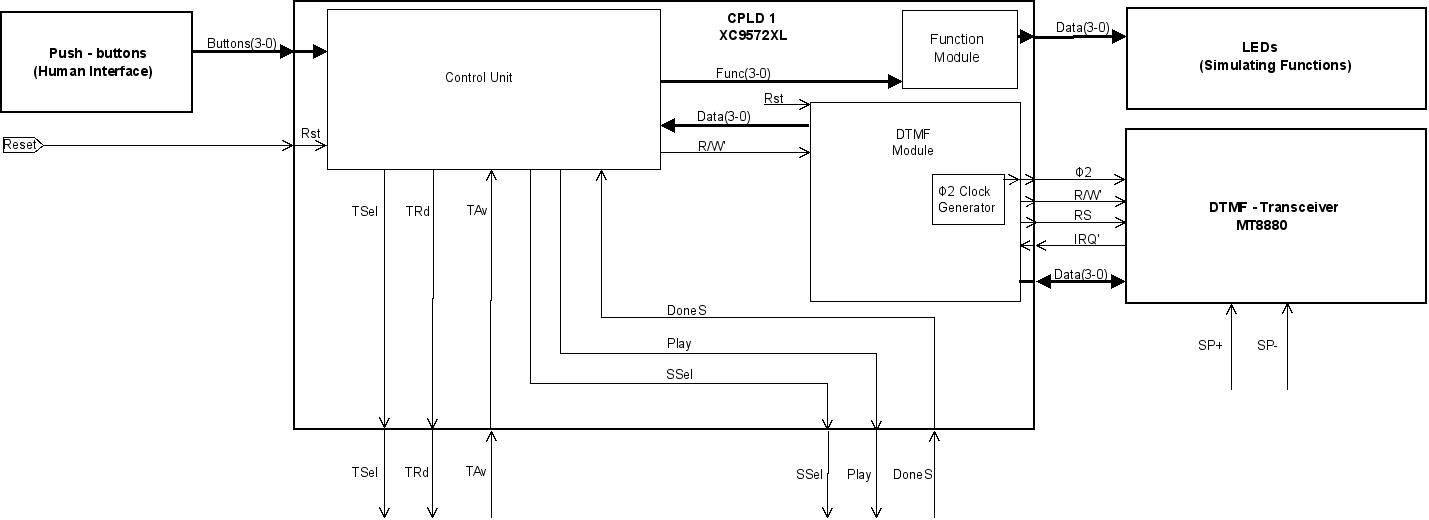
\includegraphics[scale=0.48, angle=90]{BlockDiagramCPLD1.jpg}
	  	\caption{Block Diagram (CPLD1)}
	\end{figure}

	\begin{figure}[h!]
	  \centering
	      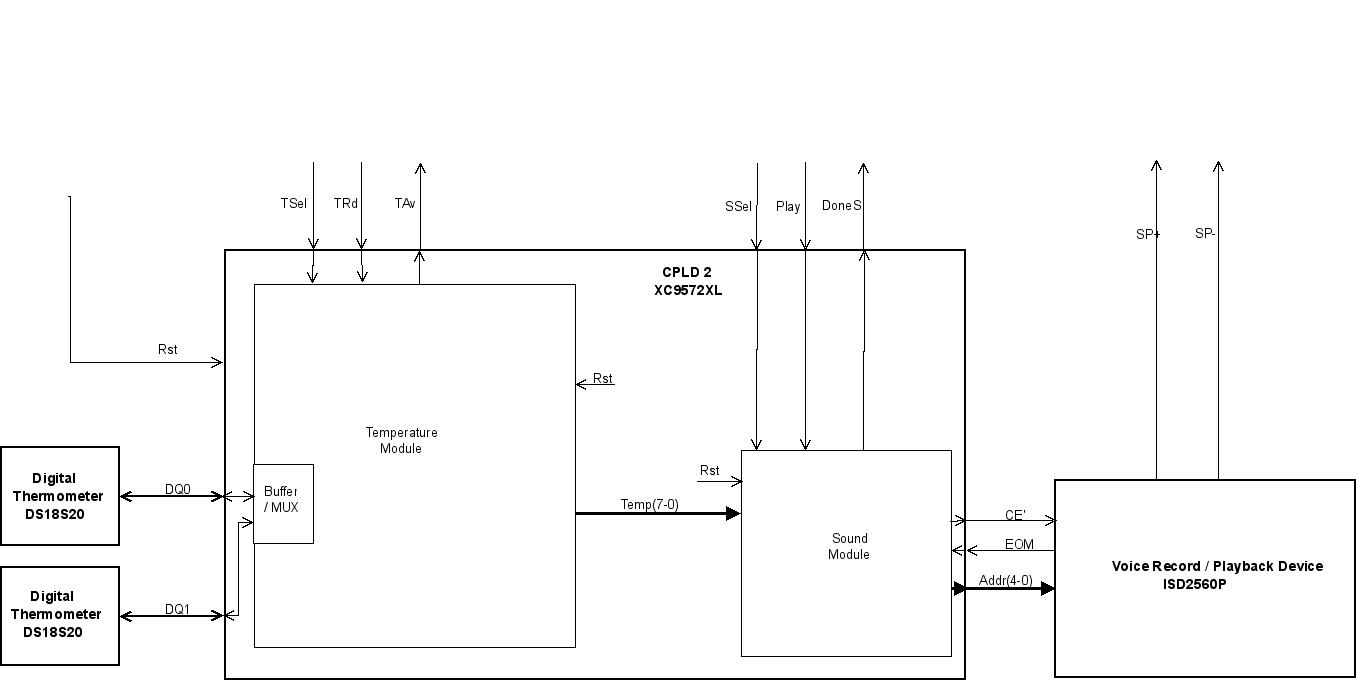
\includegraphics[scale=0.48, angle=90]{BlockDiagramCPLD2.jpg}
	  	\caption{Block Diagram (CPLD2)}
	\end{figure}


\section{Block, Functionality}

	\subsection{Data Path}

	\subsection{Control Unit}

	\subsection{Functional Modules}

		\subsubsection{DTMF Module and MT8880}
	
		\subsubsection{Sound Module and ISD2560P}

		\subsubsection{Temperature Module and DS18S20}

{\bf Purpose}

The temperature module of the CPLD is tasked with handling the serial communication with
the DS18S20 Temperature sensors via the 1-Wire buses, and outputting the read temperatures
to the sound module, allowing playback of current temperatures to the system user.\\

{\noindent \bf 1-Wire Bus}

The 1-wire buses are connected to +5V through pull-up resistors of 4.7kO , and the
two ends to the master (CPLD) and sensor (DS18S20), respectively. In its idle state, the
bus is pulled high ("weak drive") by the pull-up resistor. When sending information, the
two communicating circuits pulls the bus low by a strong logical 0 drive. \\

	\begin{figure}[h!tb]
	  \centering
	      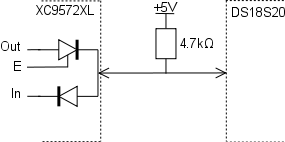
\includegraphics[scale=0.5, angle=0]{TempBus.png}
	  	\caption{Schematic of 1-Wire bus}
	\end{figure}

{\noindent \bf DS18S20 Specifics}

The temperature sensor used is the Maxim DS18S20, providing the temperature module with
9 bits of temperature resolution. The sensors used in this system are powered by an external
voltage supply of +5V, and communicated with using a 1-wire serial bus. The serial communication is
based on the master issuing Read- and Write-Timeslots. Each such slot is 60-120 us. The temperature
sensor is reset by the master pulling the bus low for at least 480 us, followed by a presence pulse
where the sensor itself pulls the bus low for 60-240 us. Following the reset, the sensor circuit accepts
a ROM-command followed by a Function-command from the master. Each command is a single byte long, and is
sent as LSB first. The master sends a zero by pulling the bus low for the whole duration of the write slot.
A one is sent by pulling the bus low for a minimum of 1 us and then releasing it for the rest of the
write slot. Between each write or read slot, a recovery period of at least 1 us is required.

When the master is done issuing commands, the DS18S20 may (depending on what commands were sent) respond
with the appropriate data. Similiarily, here the master also must issue a read-time slot by pulling the 
bus low for 1-8 us, then releasing it. The DS18S20 responds to these slots by either keeping the bus
low for a 0, or by letting the bus go high for a 1. During this time (up to 15 us after release), the
master can sample the bus. All data from the DS18S20 is sent as LSB first.\\

{\noindent \bf Read Cycle Overview}

A read cycle consists of four stages; Initialization, Command (command issuing), Receive (reading of data) and an idle state.

Initialization is performed by pulling the bus low for 512 us, then releasing the bus. The
temperature sensor responds with a presence pulse by pulling the bus low for about 106 us, confirming
its presence on the bus and its operational status. 

Detecting the presence pulse, the master starts to issue a ROM Command (Skip ROM, 0xCC), followed
by a short recovery time and then a Function Command (Convert Temperature, 0x44), according to the
read/write-timeslot method described above. The Skip ROM Command is used since the system uses only
one sensor per 1-Wire bus, and there is no need for addressing specific sensors. The Convert Temperature
command tells the DS18S20 to start converting temperature and put it in its on-chip memory for later reading.
During the conversion time (up to 750 ms), the master polls the temperature sensor by continously sending
requests by pulling the bus low for a short (4 us) period of time. The temperature sensor responds by
0 while it is busy converting, and then a 1 as soon as it is finished.
The master then resets the temperature sensor again, and follows up by sending another pair of ROM command
and Function command, 0xCC (Skip ROM) and 0xBE (Read Scratchpad), respectively. 
Ideally, the DS18S20 should now be ready to transmit the data stored on its on-chip memory of
9 bytes. Given the Read Scratchpad command, the DS18S20 now starts sending the contents of its memory
on the bus. The master goes into Receive mode and starts sampling the data by pulling the bus low,
releasing it and sampling the bus again after 4 us, all according to the process described above.
The master samples the first eight bits of data sent by the DS18S20, then another, ninth bit, the temperature sign bit, 
then gives a reset pulse to signal to the DS18S20, telling it discontinue the data transmission. 
The newly read temperature is placed on the internal (on CPLD2) temperature bus, and the temperature available signal 
(TAv) is set to 1, indicating that there is valid data on the bus, according to what was requested by the control unit.\\

{\noindent \bf Details}

The temperature modules is based around a state machine, supported by an internal Buffer/MUX as well
as a number of counters for generating timing pulses needed. \\

{\noindent \bf Buffer/MUX}

The Buffer/MUX module is directly connected to the two DS18S20 temperature sensors using 1-wire communication. The MUX is used for selecting
which of the two sensors (Sensor 0 or Sensor 1) is to be communicated with, and uses the TSel input signal.
the buffer is a tri-state buffer with an enable signal, E. When E is set to 1, the selected (by TSel) 1-wire bus
is used as an output signal from the master. When E is set to 0, the master can read data from the bus.\\

{\noindent \bf Counters}

Internally, the temperature module uses a number of counters.\\

{\noindent \bf State Machine}
	
For a complete description of the internal state machine used by the temperature module, see the section
on state machines.\\

		\subsubsection{Control Functions}

		\subsubsection{Interface}

\section{State Machines}
		\subsubsection{DS18S20 Serial Communication}
			(Refering to State Diagram for Temperature Module)
			Reset: All signals and counters are reset to their default (start-) values.
			Defaults: By default, all signals retain their old values.
			Initialization (States 0-3):
				State 0 : Idle State and Reset Point. The temperature module waits
						in a loop until it receives a logical one on TRd (Temperature Read).
						On TRd = 1, the state machines starts running, setting TAv = 0,
						because the read cycle is now running, and the data on the temperature
						output bus is no longer valid.
				State 1 : Delay state, waits for pulse on DelayLong (512 us), then goes to state 2.
				State 2 : Master pulls bus low for 512 us and sets data to 0xCC (Skip ROM), then goes to state 3.
				State 3 : Master releases bus, allowing the DS18S20 to send a presence pulse. Waits 512 us.
			Write (States 4-8):
				State 4 : Preparation state, master prepares to send and goes to state 5 after 16 us.
				State 5 : Main Send state, master determines what bit is to be sent next (according to bitCnt).
				State 6 : Between bits, recovery state. Determines if there are more bits to be sent in the current
					  byte, according to BitCnt. If so, goes back to state 5. If not, continues to state 7.
				State 7 : Determines if the DS18S20 is currently converting temperature. If it is, 
					  

		\subsubsection{MT8880}
		\subsubsection{ISD2560P}

\section{Timing Diagrams}

\section{Fault Analysis}

\section{Appendix}

	\subsection{List of Components}

	\subsection{Circuit diagram}

	\subsection{PCB Layout}

	\subsection{Program listings}

	\subsection{List of Signals}

\end{document}
